\documentclass{standalone}
\usepackage{tikz}
\usepackage{ctex,siunitx}
\setCJKmainfont{Noto Serif CJK SC}
\usepackage{tkz-euclide}
\usepackage{amsmath}
\usetikzlibrary{patterns, calc}
\usetikzlibrary {decorations.pathmorphing, decorations.pathreplacing, decorations.shapes}
\pgfdeclareverticalshading{pile}{100bp}{
  color(0bp)=(black);color(50bp)=(white);color(100bp)=(black)
}
\pgfdeclareverticalshading{pile2}{100bp}{
  color(0bp)=(white);color(50bp)=(black);color(100bp)=(white)
}
\begin{document}
\small
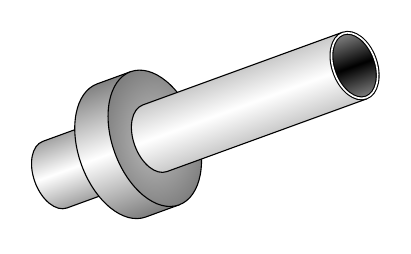
\begin{tikzpicture}[>=latex, scale=0.9,rotate=20]
  % \useasboundingbox(0.9,0)rectangle(5.1,5);
  \draw [shading=pile,shading angle=20] (0,0.5) arc(90:270:0.3 and 0.5)--(1,-0.5)--(1,0.5)--cycle;
  \draw [shading=pile,shading angle=20] (1,1) arc(90:270:0.6 and 1)--(1.5,-1)--(1.5,1)--cycle;
  \draw[inner color=lightgray,outer color=gray](1.5,0)ellipse(0.6 and 1);
  \draw [shading=pile,shading angle=20] (1.5,0.5) arc(90:270:0.3 and 0.5)--(4.5,-0.5)arc(270:90:0.3 and 0.5)--cycle;
  \draw[double,shading=pile2,shading angle=20](4.5,0)ellipse(0.3 and 0.48);
\end{tikzpicture}
\end{document}